\section{Auswertung}
\label{sec:Auswertung}
Im Verlauf des Versuchs sind vier verschiedene Messreihen zur Untersuchung der Halbwertzeit verschiedener Isotope.
Die entsprechenden Messwerte sind in Tabelle \ref{tab:Mess1} und \ref{tab:Mess2} aufgelistet. 
Die erste Spalte misst die Hintergrundaktivität, indem in 30 Sekunden Intervallen die Zerfallsanzahl detektiert wird.
Die zweite Spalte stellt die gemessenen Zerfälle von Vanadium in 35 Sekunden Intervallen dar, während die dritte und
vierte Spalte den Zerfall der Silberisotope \isotope[108]{Ag} und \isotope[110]{Ag} in 10 beziehungsweise
8 Sekunden Intervallen dokumentiert.
\begin{table}[H]
  \centering
  \caption{Gemessene Zerfälle für verschiedene Isotope in festen Zeitintervallen.}
  \label{tab:Mess1}
  \begin{tabular}{S[table-format=2] S[table-format=3] S[table-format=3] S[table-format=3]}
      \toprule
      {Nullmessung $\Delta t=30s$ }&{\isotope[52]{V}: $\Delta t=35s$}&{\isotope[108]{Ag}/\isotope[110]{Ag}: $\Delta t=10s$}&{\isotope[108]{Ag}/\isotope[110]{Ag}: $\Delta t=8s$}\\
      \midrule
      12 & 221 & 313 & 174 \\
      13 & 184 & 49 & 137 \\
      8 & 183 & 65 & 119 \\
      16 & 153 & 41 & 104 \\
      9 & 129 & 40 & 66 \\
      13 & 134 & 32 & 65 \\
      11 & 134 & 34 & 57 \\
      7 & 106 & 34 & 45 \\
      15 & 103 & 28 & 47 \\
      13 & 99 & 17 & 31 \\
      9 & 85 & 17 & 27 \\
      9 & 70 & 21 & 32 \\
      10 & 69 & 16 & 28 \\
      10 & 59 & 25 & 16 \\
      9 & 58 & 15 & 31 \\
      11 & 56 & 19 & 21 \\
      7 & 48 & 24 & 21 \\
       & 49 & 14 & 21 \\
       & 35 & 26 & 9 \\
       & 31 & 9 & 11 \\
       & 33 & 22 & 11 \\
       & 28 & 16 & 16 \\
       & 26 & 18 & 7 \\
       & 26 & 16 & 14 \\
       & 37 & 8 & 10 \\
       & 18 & 16 & 12 \\
       & 22 & 11 & 13 \\     
      \bottomrule
  \end{tabular}
\end{table}

\begin{table}[H]
  \centering
  \caption{Gemessene Zerfälle für verschiedene Isotope in festen Zeitintervallen.}
  \label{tab:Mess2}
  \begin{tabular}{S[table-format=2] S[table-format=3] S[table-format=3] S[table-format=3]}
      \toprule
      {Nullmessung $\Delta t=30s$ }&{\isotope[52]{V}: $\Delta t=35s$}&{\isotope[108]{Ag}/\isotope[110]{Ag}: $\Delta t=10s$}&{\isotope[108]{Ag}/\isotope[110]{Ag}: $\Delta t=8s$}\\
      \midrule
      &  & 14 & 13 \\
      &  & 13 & 8 \\
      &  & 15 & 15 \\
      &  & 11 & 15 \\
      &  & 8 & 11 \\
      &  & 12 & 17 \\
      &  & 11 & 10 \\
      &  & 9 & 9 \\
      &  & 16 & 12 \\
      &  & 11 & 11 \\
      &  & 9 & 11 \\
      &  & 8 & 5 \\
      &  & 18 & 4 \\
      &  & 5 & 6 \\
      &  & 9 & 5 \\
      &  & 13 & 6 \\
      &  & 15 & 7 \\
      &  &  & 10 \\
      &  &  & 7 \\
      &  &  & 8 \\
      &  &  & 6 \\
      &  &  & 8 \\
      &  &  & 5 \\
      &  &  & 3 \\
      &  &  & 4 \\       
      \bottomrule
  \end{tabular}
\end{table}
\noindent Nun müssen zunächst der Fehler der gemessenen Zerfallsanzahl bestimmt werden. Dieser ergibt sich dieser nach der 
Poissonverteilung zu $\sqrt{N}$, wobei $N$ die gemessene Anzahl an Zerfällen im entsprechenden Zeitintervall angibt.
Nun müssen die gemessenen Zerfälle noch um die natürliche Hintergrundstrahlung bereinigt werden. Da diese mit der Messung des entsprechenden Isotopenzerfalls
nichts zu tun hat, aber immer auftritt. Die Hintergrundaktivität ergibt sich aus der Summe aller Zerfälle $N_\text{gesamt}$ über alle Intervalle, geteilt durch die gesamte Messzeit$T_\text{gesamt}$.
Damit ergibt sich 
\begin{equation*}
  A=\frac{N_\text{geamt}}{T_\text{gesamt}}=\frac{N_\text{geamt}}{17\cdot \qty{30}{s}}=\frac{182}{\qty{510}{s}}=\qty{0.357}{\per\s}
\end{equation*}
Der Fehler der Aktivität ergibt sich über den Fehler der Zerfallsanzahl $dN_\text{gesamt}=\sqrt{N_\text{gesamt}}$ zu $dA=A\cdot \frac{dN_\text{gesamt}}{N_\text{gesamt}}=\qty{0.026}{\per\s}$.
Damit lässt sich die Hintergrundaktivität als $A_\text{Hint}=\qty{0.357(0.026)}{\per\s}$ angeben.
Im Folgenden wird die Fehlerrechnung mit der Python Bibliothek Uncertainties \cite{uncertainties} durchgeführt.
Wenn nun die Hintergrundaktivität von den Isotopenmessungen unter Berücksichtigung des Fehlers abgezogen wird,
ergeben sich die Messwerte aus Tabelle \ref{tab:Korr1} und \ref{tab:Korr2}.
\begin{table}[H]
  \centering
  \caption{Korrigierte Zerfälle unter Berücksichtigung des Messfehlers und der Hintergrundaktivität.}
  \label{tab:Korr2}
  \begin{tabular}{c c c}
      \toprule
      {\isotope[52]{V}: $\Delta t=35s$}&{\isotope[108]{Ag}/\isotope[110]{Ag}: $\Delta t=10s$}&{\isotope[108]{Ag}/\isotope[110]{Ag}: $\Delta t=8s$}\\
      \midrule
      $208,51 \pm 14,89$ & $309,43 \pm 17,69$ & $171,15 \pm 13,19$ \\
      $171,51 \pm 13,60$ & $45,43 \pm 7,00$ & $134,15 \pm 11,71$ \\
      $170,51 \pm 13,56$ & $61,43 \pm 8,07$ & $116,15 \pm 10,91$ \\
      $140,51 \pm 12,40$ & $37,43 \pm 6,41$ & $101,15 \pm 10,20$ \\
      $116,51 \pm 11,40$ & $36,43 \pm 6,33$ & $63,15 \pm 8,13$ \\
      $121,51 \pm 11,61$ & $28,43 \pm 5,66$ & $62,15 \pm 8,07$ \\
      $121,51 \pm 11,61$ & $30,43 \pm 5,84$ & $54,15 \pm 7,55$ \\
      $93,51 \pm 10,34$ & $30,43 \pm 5,84$ & $42,15 \pm 6,71$ \\
      $90,51 \pm 10,19$ & $24,43 \pm 5,30$ & $44,15 \pm 6,86$ \\
      $86,51 \pm 9,99$ & $13,43 \pm 4,13$ & $28,15 \pm 5,57$ \\
      $72,51 \pm 9,27$ & $13,43 \pm 4,13$ & $24,15 \pm 5,20$ \\
      $57,51 \pm 8,42$ & $17,43 \pm 4,59$ & $29,15 \pm 5,66$ \\
      $56,51 \pm 8,36$ & $12,43 \pm 4,01$ & $25,15 \pm 5,30$ \\
      $46,51 \pm 7,74$ & $21,43 \pm 5,01$ & $13,15 \pm 4,01$ \\
      $45,51 \pm 7,67$ & $11,43 \pm 3,88$ & $28,15 \pm 5,57$ \\
      $43,51 \pm 7,54$ & $15,43 \pm 4,37$ & $18,15 \pm 4,59$ \\
      $35,51 \pm 6,99$ & $20,43 \pm 4,91$ & $18,15 \pm 4,59$ \\
      $36,51 \pm 7,06$ & $10,43 \pm 3,75$ & $18,15 \pm 4,59$ \\
      $22,51 \pm 5,99$ & $22,43 \pm 5,11$ & $6,15 \pm 3,01$ \\
      $18,51 \pm 5,64$ & $5,43 \pm 3,01$ & $8,15 \pm 3,32$ \\
      $20,51 \pm 5,82$ & $18,43 \pm 4,70$ & $8,15 \pm 3,32$ \\
      $15,51 \pm 5,37$ & $12,43 \pm 4,01$ & $13,15 \pm 4,01$ \\
      $13,51 \pm 5,18$ & $14,43 \pm 4,25$ & $4,15 \pm 2,65$ \\
      $13,51 \pm 5,18$ & $12,43 \pm 4,01$ & $11,15 \pm 3,75$ \\
      $24,51 \pm 6,15$ & $4,43 \pm 2,84$ & $7,15 \pm 3,17$ \\
      $5,51 \pm 4,34$ & $12,43 \pm 4,01$ & $9,15 \pm 3,47$ \\
      $9,51 \pm 4,78$ & $7,43 \pm 3,33$ & $10,15 \pm 3,61$ \\
      \bottomrule
  \end{tabular}
\end{table}
\begin{table}[H]
  \centering
  \caption{Korrigierte Zerfälle unter Berücksichtigung des Messfehlers und der Hintergrundaktivität.}
  \label{tab:Korr1}
  \begin{tabular}{c c c}
      \toprule
      {\isotope[52]{V}: $\Delta t=35s$}&{\isotope[108]{Ag}/\isotope[110]{Ag}: $\Delta t=10s$}&{\isotope[108]{Ag}/\isotope[110]{Ag}: $\Delta t=8s$}\\
      \midrule
      & $10,43 \pm 3,75$ & $10,15 \pm 3,61$ \\
      & $9,43 \pm 3,62$ & $5,15 \pm 2,84$ \\
      & $11,43 \pm 3,88$ & $12,15 \pm 3,88$ \\
      & $7,43 \pm 3,33$ & $12,15 \pm 3,88$ \\
      & $4,43 \pm 2,84$ & $8,15 \pm 3,32$ \\
      & $8,43 \pm 3,47$ & $14,15 \pm 4,13$ \\
      & $7,43 \pm 3,33$ & $7,15 \pm 3,17$ \\
      & $5,43 \pm 3,01$ & $6,15 \pm 3,01$ \\
      & $12,43 \pm 4,01$ & $9,15 \pm 3,47$ \\
      & $7,43 \pm 3,33$ & $8,15 \pm 3,32$ \\
      & $5,43 \pm 3,01$ & $8,15 \pm 3,32$ \\
      & $4,43 \pm 2,84$ & $2,15 \pm 2,25$ \\
      & $14,43 \pm 4,25$ & $1,15 \pm 2,01$ \\
      & $1,43 \pm 2,25$ & $3,15 \pm 2,46$ \\
      & $5,43 \pm 3,01$ & $2,15 \pm 2,25$ \\
      & $9,43 \pm 3,62$ & $3,15 \pm 2,46$ \\
      & $11,43 \pm 3,88$ & $4,15 \pm 2,65$ \\
      &  & $7,15 \pm 3,17$ \\
      &  & $4,15 \pm 2,65$ \\
      &  & $5,15 \pm 2,84$ \\
      &  & $3,15 \pm 2,46$ \\
      &  & $5,15 \pm 2,84$ \\
      &  & $2,15 \pm 2,25$ \\
      &  & $0,15 \pm 1,74$ \\
      &  & $1,15 \pm 2,01$ \\
      \bottomrule
  \end{tabular}
\end{table}

\noindent Die korrigierten Messwerte können nun dazu benutzt werden, dass Zerfallsgesetz zu bestätigen.
Dafür werden die Daten logarithmiert, also der $\ln{N}$ genommen. Dann ergibt sich
nach der Theorie ein linearer Zusammenhang
\begin{equation}
    \ln{N(t)}=\ln{N_0(1-e^{-\lambda \Delta t})}-\lambda t
    \label{eq:linN}
\end{equation}
Für Vanadium ist diese Auswertung direkt mit Polyfit aus der Bibliothek Numpy \cite{numpy}
durchführbar, wobei die Fehler der einzelnen Messpunkte als Gewichte der Form $1/d\ln{N}$ übergeben werden. Dadurch werden 
Messpunkte mit einem geringeren relativen Fehler mehr beachtet als welche, wo der relative Fehler von $N$ groß ist.
Für Vanadium ergeben sich die Ausgleichskoeffizienten zu
\begin{align*}
  \lambda_V&=\qty{3.1(0.1)e-3}{\per\s}\\
  \ln{N_0(1-e^{-\lambda \Delta t})}_V&=\num{5.43(0.03)}\frac{1}{\ln{s}}.
\end{align*}
Die Halbwertzeit von Vanadium ist nach Formel \eqref{eq:} dann $T_V=\qty{224(7)}{\second}$.
Datenpunkte und Ausgleichsgerade sind in Abbildung \ref{fig:Van} eingezeichnet.\\
\\
\noindent Die Bestimmung der Halbwertzeit von \isotope[108]{Ag} und \isotope [110]{Ag} läuft vom Prinzip
ab wie bei Vanadium. Der große Unterschied besteht darin, dass die Zerfälle zeitweise Parallel ablaufen.
Der Zerfall von \isotope [110]{Ag} läuft sehr schnell ab, weswegen erst der lang andauernde Zerfall von \isotope [108]{Ag}
untersucht wird und dann ausgehend von der ermittelten zeitlichen Entwicklung
des Zerfalls können dann die erwarteten Zerfälle von \isotope [108]{Ag} von den Datenpunkten
abgezogen werden und so eine Ausgleichsrechnung mit den bereinigten Daten durchzuführen und die Halbwertzeiten des anderen Zerfalls 
herauszufinden. Die um die Hintergrundstrahlung korrigierten Datenpunkte der 
ersten Messung für Silber sind in Abbildung \ref{fig:Si1} dargestellt. Die Wahl des ersten Datenpunktes der zur Regression des Zerfalls von \isotope [108]{Ag}, sollte
so gewählt werden, dass davon ausgegangen werden kann, dass der Zerfall des kurzlebigen Zerfalls bereits abgeklungen ist. Dieser Punkt ist in der Abbildung grün markiert.
Die Lineare Ausgleichsrechnung ergibt dann
\begin{align*}
  \lambda_\text{\isotope[108]{Ag}}&=\qty{1.6(1.0)e-3}{\per\s}\\
  \ln{N_0(1-e^{-\lambda \Delta t})}_\text{\isotope[108]{Ag}}&=\num{2.85(0.32)}\frac{1}{\ln{s}}.
\end{align*}
Als Halbwertzeit ergibt sich $T_\text{\isotope[108]{Ag}}=\qty{422(256)}{\second}$.

\begin{align*}
  \lambda_\text{\isotope[110]{Ag}}&=\qty{3.3(0.6)e-2}{\per\s}\\
  \ln{N_0(1-e^{-\lambda \Delta t})}_\text{\isotope[110]{Ag}}&=\num{2.91(0.259)}\frac{1}{\ln{s}}.
\end{align*}
$T_\text{\isotope[110]{Ag}}=\qty{20.9(3.91)}{\second}$
\begin{align*}
  \lambda_\text{\isotope[108]{Ag}}&=\qty{4.4(1.3)e-3}{\per\s}\\
  \ln{N_0(1-e^{-\lambda \Delta t})}_\text{\isotope[108]{Ag}}&=\num{3.33(0.35)}\frac{1}{\ln{s}}.
\end{align*}
$T_\text{\isotope[108]{Ag}}=\qty{156(44)}{\second}$
\begin{align*}
  \lambda_\text{\isotope[110]{Ag}}&=\qty{1.8(0.1)e-2}{\per\s}\\
  \ln{N_0(1-e^{-\lambda \Delta t})}_\text{\isotope[110]{Ag}}&=\num{1.93(0.05)}\frac{1}{\ln{s}}.
\end{align*}
$T_\text{\isotope[110]{Ag}}=\qty{38.9(2.41)}{\second}$
\begin{figure}[H]
  \centering
  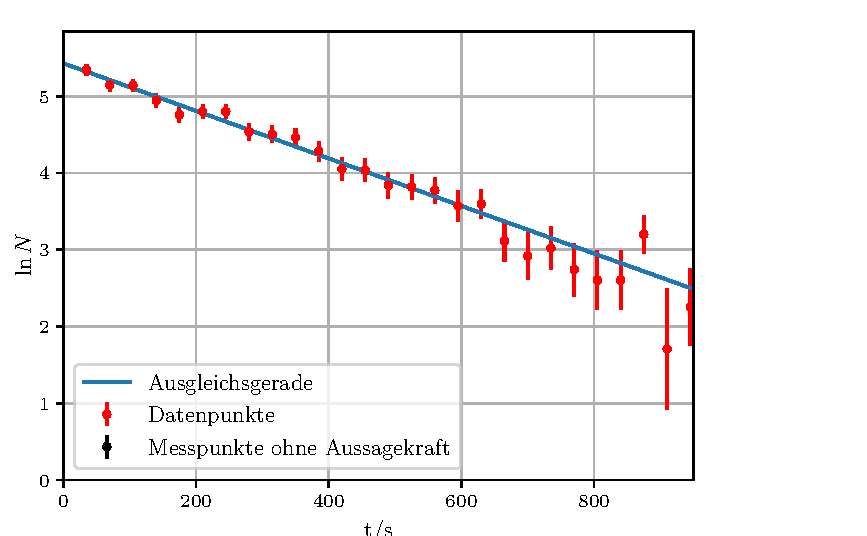
\includegraphics{build/Vanadium.pdf}
  \caption{Logarithmische Auftragung der Zerfälle von Vanadium in 35s Intervallen.}
  \label{fig:Van}
\end{figure}

\begin{figure}[H]
  \centering
  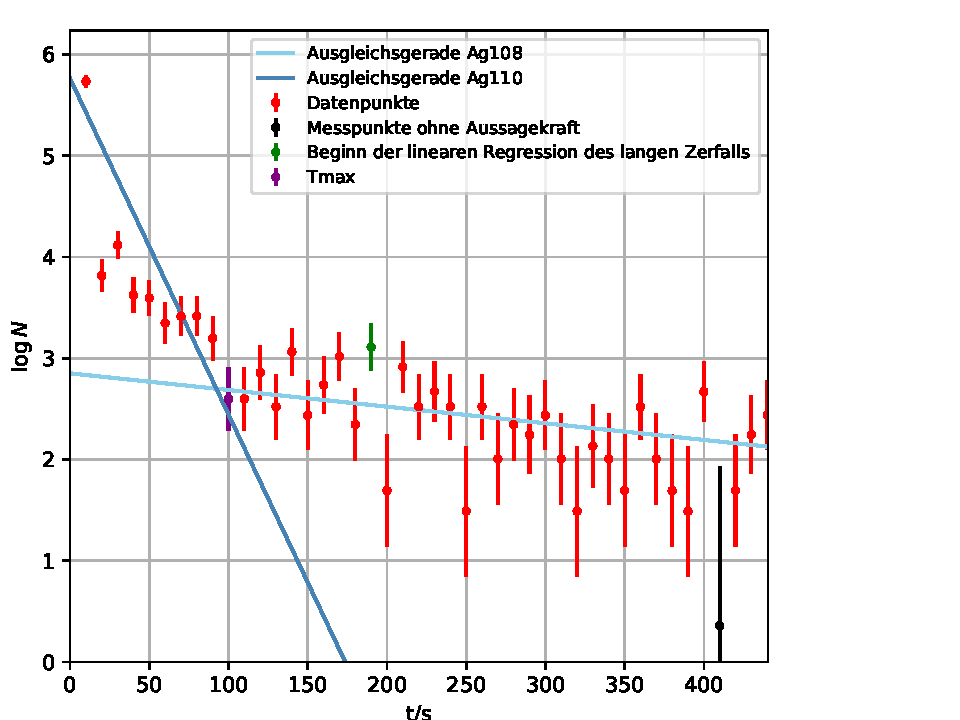
\includegraphics{build/Silber1.pdf}
  \caption{Logarithmische Auftragung der Zerfälle von Silber in 10s Intervallen.}
  \label{fig:Si1}
\end{figure}

\begin{figure}[H]
  \centering
  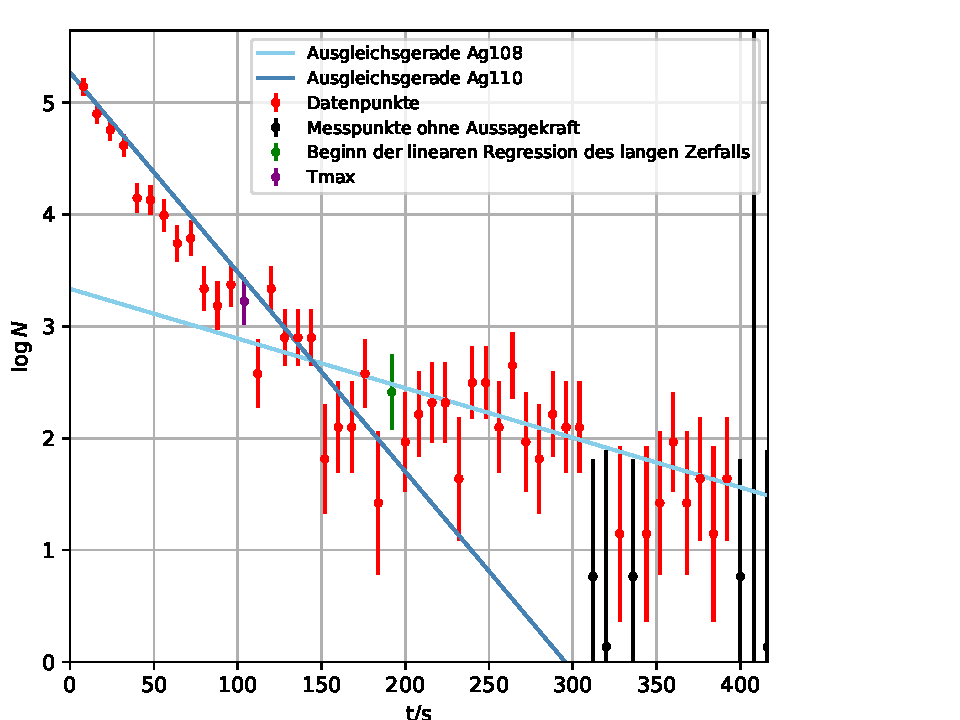
\includegraphics{build/Silber2.pdf}
  \caption{Logarithmische Auftragung der Zerfälle von Silber in 8s Intervallen.}
  \label{fig:Si2}
\end{figure}

